% !TeX root = ./main.tex

\documentclass[fleqn,10pt]{wlscirep}
\usepackage[utf8]{inputenc}
\usepackage[T1]{fontenc}
\title{SPIDIA blood stabilization study: Substantial activation of gene expression is mediated by blood incubation in EDTA tubes}


\author[1,*]{Vlasta Korenková}
\author[2]{Hui Zhang}
\author[3]{Lucie Žáčková}
\author[4]{Robert Sjöback}
\author[4]{Jens Björkman}
\author[5]{David Švec}
\author[6]{Sara Pizzamiglio}
\author[6]{Chiara Maura Ciniselli}
\author[7]{Mogens Kruhøffer}
\author[8]{Ralf Wyrich}
\author[8]{Uwe Ölmüller}
\author[9]{Edith Rian}
\author[10]{Vendula Novosadová}
\author[11]{Mikael Kubista}
\author[12]{Veronika Vymetalková}
\author[6]{Paolo Verderio}

\affil[1]{Charles University, First Faculty of Medicine, Institute of Immunology and Microbiology, Prague, 128 00, Czech Republic}
\affil[*]{vlasta.korenkova@lf1.cuni.cz}
\affil[2]{Thermo Fisher Scientific, Oslo, 0379, Norway}
\affil[3]{Institute of Biotechnology of the Czech Academy of Sciences, Vestec, 252 50, Czech Republic}
\affil[4]{RISE Research Institutes of Sweden, Division of Bioscience and Materials, Gothenburg, 402 29, Sweden}
\affil[5]{SOTIO Biotech, Prague, 180 00, Czech Republic}
\affil[6]{Fondazione IRCCS Istituto Nazionale dei Tumori, Department of Experimental Oncology, Milan, 20133, Italy}
\affil[7]{Aarhus University Hospital, Department of Molecular Medicine, Aarhus, 8200, Denmark}
\affil[8]{QIAGEN GmbH, Hilden, 40724, Germany}
\affil[9]{Rösslyng GmbH, Bonn, 53111, Germany}
\affil[10]{Institute of Molecular Genetics of the Czech Academy of Sciences, Laboratory of Cell Differentiation, BIOCEV, Vestec, 252 50, Czech Republic}
\affil[11]{Institute of Biotechnology of the Czech Academy of Sciences, Laboratory of Gene Expression, Vestec, 252 50, Czech Republic}
\affil[12]{Institute of Experimental Medicine of the Czech Academy of Sciences, Department of Molecular Genetics, Prague, 142 20, Czech Republic}



%\affil[+]{these authors contributed equally to this work}

%\keywords{Preanalytical phase, EDTA tubes, PAXgene tubes, mRNA, gene expression, quality of samples, degradation}

\begin{abstract}
    Example Abstract. Abstract must not include subheadings or citations. Example Abstract. Abstract must not include subheadings or citations. Example Abstract. Abstract must not include subheadings or citations. Example Abstract. Abstract must not include subheadings or citations. Example Abstract. Abstract must not include subheadings or citations. Example Abstract. Abstract must not include subheadings or citations. Example Abstract. Abstract must not include subheadings or citations. Example Abstract. Abstract must not include subheadings or citations.
    \end{abstract}


\begin{document}

\flushbottom
\maketitle
% * <john.hammersley@gmail.com> 2015-02-09T12:07:31.197Z:
%
%  Click the title above to edit the author information and abstract
%
\thispagestyle{empty}

\noindent Please note: Abbreviations should be introduced at the first mention in the main text – no abbreviations lists. Suggested structure of main text (not enforced) is provided below.

\section*{Introduction}
The Introduction section, of referenced text\cite{Figueredo:2009dg} expands on the background of the work (some overlap with the Abstract is acceptable). The introduction should not include subheadings.

\section*{Results}
%Up to three levels of \textbf{subheading} are permitted. Subheadings should not be numbered.

\subsection*{Subsection}

Example text under a subsection. Bulleted lists may be used where appropriate, e.g.

\begin{itemize}
\item First item
\item Second item
\end{itemize}

\subsubsection*{Third-level section}
 
Topical subheadings are allowed.

\section*{Discussion}
%The Discussion should be succinct and must not contain subheadings.

\section*{Methods}
%
\subsection*{Study design}
This study (Figure 1) was performed in several phases: (1) the pre-validation phase with a small number of samples,  including all candidate markers; (2) the extended validation phase with a larger number of samples and only selected candidate markers; and (3) the confirmatory phase using clinical samples and only selected candidate markers. 

\subsubsection*{Pre-validation study}
In the pre-validation study, 72 primers and 24 probes (Table S1) were tested for their ability to detect ongoing RNA degradation or deregulation in a limited number of blood samples (6 samples from healthy donors) with good precision using qPCR. Blood samples were incubated in EDTA tubes for 0, 2, 6, 24, 48, and 72 hours at RT. Blood samples from the same donors were incubated in PAXgene tubes for 2, 24, 48, and 72 hours at both RT and 30°C. The results were statistically analyzed, and the selected candidate assays were subsequently used in the extended validation study.

\subsubsection*{Extended validation study}
Samples obtained from a large cohort of healthy donors were incubated in EDTA tubes for 0, 24, and 48 hours at RT (60 samples). A portion of these blood samples was incubated in PAXgene tubes, with 20 samples incubated at RT for 2, 48, and 72 hours, and 40 samples incubated at 30°C for the same time points. The potential biomarkers were then subjected to statistical analysis and validated.

\subsubsection*{EDTA application test}
A confirmatory application test was conducted to assess the overall ability of the selected biomarkers to detect variations in sample treatment in EDTA blood tubes. This test was performed using 69 samples from patients with colorectal carcinoma.

\subsection*{Blood collection and ethics statement}
Whole blood samples were collected from healthy adult subjects using standard phlebotomy techniques in both K2EDTA (EDTA) tubes (BD) and PAXgene Blood RNA Tubes (PAXgene, PreAnalytiX). The number of tubes and the volume of blood collected for each part of study are described in the study design (Figure 1). All participants provided written informed consent, and the study was approved by the Norwegian South East Regional Committee for Medical and Health Research Ethics (REC South East), in accordance with the 2013 Helsinki Declaration (citace).

\subsection*{RNA isolation from whole blood collected into RNA PAXgene tubes}
For each subject, 2.5 mL of whole blood collected in the PAXgene tubes, was incubated for 2 hours at RT according to the manufacturer's instructions. RNA from blood collected in PAXgene tubes was extracted using the PAXgene Blood RNA Kit (QIAGEN) following the manufacturer's protocol. After isolation, RNA was stored at –80°C (T0). Additionally, four other PAXgene tubes were incubated for 48 hours (T48) and 72 hours (T72) at 30°C and RT, respectively (Table S2). Since PAXgene tubes are validated for transport and storage of blood specimens for up to three days at 18°C–25°C (citace), we considered the elevated storage temperature as a relevant simulation of off-label, improper specimen handling. 

\subsection*{RNA isolation from whole blood collected into EDTA tubes}
For the same subjects, blood was also collected in EDTA tubes in parallel. To minimize tube-related bias in the study, 2.5 mL of blood collected in EDTA tubes were transferred into PAXgene tubes at the specified incubation times: EDTA control T0 immediatally after collection and two additional EDTA tubes were transferred after 24 hour incubation and 48 hour incubation at RT, respectively. RNA was isolated using the PAXgene Blood RNA Kit (QIAGEN).

For the confirmatory study, blood samples were collected in EDTA tubes only. According to the protocols from Slyskova (citace), RNA isolation was conducted as soon as possible after collection, within 6 hours. Total RNA was isolated using TRIzol (Invitrogen) (Table S3).  

\subsection*{cDNA synthesis}
Before cDNA synthesis, RNA quantity was measured with Nanodrop spectrophotometer ND-1000 (Thermo Scientific), and RNA integrity was assessed using an Agilent 2100 Bioanalyzer (Agilent Technologies).

For qPCR assay development, cDNA synthesis was performed with SuperScript III First-Strand Synthesis System (Life Technologies) with random hexamers. Manufacturer’s  instructions were followed, using 1 µg of RNA per sample in a 100 µL reaction, with the resulting cDNA diluted 1:10 before PCR setup. 

For precision, pre-validation and validation studies, cDNA synthesis was performed using ABI High Capacity cDNA Reverse Transcription (Life Technologies) with random hexamers, in 20 µL reactions using 200 ng RNA extracted from blood. Reverse transcription was conducted under standard conditions as described in the manufacturer's manual, and the resulting cDNA was diluted 1:1 before further processing. 

For the confirmatory study, cDNA was synthesized from 0.5 µg of RNA in 20 µL reactions using the RevertAidTM First strand cDNA synthesis kit with random hexamers (Fermentas), and the cDNA was diluted 1:10 prior to qPCR setup.

\subsection*{Differentially expressed candidate mRNA quality biomarker design}
Differentially expressed candidate mRNA quality biomarkers were selected from a previously published microarray study using Affymetrix microarray data (Affymetrix GeneChip U133 Plus 2.0 cartridge) with RNA NuGEN labeling procedures (Zhang 2014). The results highlighted RNA species that demonstrated the most significant changes in gene expression during the studied storage period.

qPCR assays with probes were designed as medium (M) and short (S) assays. Both assays contained a common forward primer and a variable reverse primer. EDTA assays for upregulation included CD69, PHF1, FCGR3A, CXCR1, STEAP4, while EDTA assays for downregulation included TLR8, CXCR2, BTG3, CD83, JUN, ERMN. The reference genes used for EDTA samples were GAPDH S, GUSB S, PPIB S. PAXgene assays for degradation inluded MAGT1, EIF3, IFNGR1, GNG2, RLIM, RCHY1, RAD17, while PAXgene candidates for reference genes included SCARNA10, OAZ1, FKBP8. 

Primer design was carried out using Primer BLAST (reference), and probe design was conducted with Beacon Designer (PREMIER Biosoft International). All assays were designed to span at least one intron and/or to have one primer covering an exon/exon boundary. 

Assay criteria included linearity within a 5-log dynamic range, LC480 error < 0.2 (LC480 error is the mean square error of the single data points fit to the regression line), efficiency (80% < efficiency < 105%), specificity (no amplification of gDNA or ≥ 5 cycles difference between target and genomic Cq-value), and no amplification of No Template Controls (NTCs). All assays (10 µL reaction volume) were evaluated with the QuantiTect SYBR Green PCR Kit and QuantiTect Probe PCR Kit (Qiagen) on the LightCycler 480 (Roche), Realplex (Eppendorf), and Rotor-Gene 6000 (Qiagen). 

The QuantiTect SYBR run protocol involved activation at 95°C for 15 minutes, amplification at 95°C for 15 seconds, 57°C for 30 seconds, and 72°C for 30 seconds (45 cycles), with a melting curve temperature range of 60–95°C. The QuantiTect Probe run protocol included activation at 95°C for 15 minutes, amplification at 95°C for 15 seconds, and 61°C for 60–120 seconds (50 cycles). All assays were initially evaluated using SYBR green chemistry to test the primers. After primer approval, a hydrolysis probe was designed and assessed as described for the primers. The annealing temperature was set to 60°C in silico and evaluated experimentally with a temperature gradient test. The optimal annealing temperature was determined to be 57°C for SYBR chemistry primers and 61°C for hydrolysis probe chemistry. Information on all primers and their validation is included in Table S1.

\subsection*{qPCR analysis}
For PAXgene biomarker validation study, all assays were run using QuantiTect Probe PCR Kit (Qiagen): activation at 95°C for 15 minutes, amplification at 95°C for 15 seconds and 61°C for 90 seconds (40 cycles), with 2 µL of cDNA in a 20 µL total volume in the 7900HT Fast Real-Time PCR System (Applied Biosystems). Each sample was run in technical triplicates. Candidate biomarker assays were selected based on the type of collection tube (EDTA or PAXgene) and applied to the corresponding blood samples. Reverse transcription controls and NTCs were included for all assays throughout the process. Reference gene candidates were determined using Normfinder (GenEx, MultiD Analyses). All data were preprocessed in GenEx Enterprise (MultiD Analyses).

\subsection*{Gene-specific preamplification for high-throughput qPCR}

\bibliography{sample}

\noindent LaTeX formats citations and references automatically using the bibliography records in your .bib file, which you can edit via the project menu. Use the cite command for an inline citation, e.g.  \cite{Hao:gidmaps:2014}.

For data citations of datasets uploaded to e.g. \emph{figshare}, please use the \verb|howpublished| option in the bib entry to specify the platform and the link, as in the \verb|Hao:gidmaps:2014| example in the sample bibliography file.

\section*{Acknowledgements (not compulsory)}

Acknowledgements should be brief, and should not include thanks to anonymous referees and editors, or effusive comments. Grant or contribution numbers may be acknowledged.

\section*{Author contributions statement}

Must include all authors, identified by initials, for example:
A.A. conceived the experiment(s),  A.A. and B.A. conducted the experiment(s), C.A. and D.A. analysed the results.  All authors reviewed the manuscript. 

\section*{Additional information}

To include, in this order: \textbf{Accession codes} (where applicable); \textbf{Competing interests} (mandatory statement). 

The corresponding author is responsible for submitting a \href{http://www.nature.com/srep/policies/index.html#competing}{competing interests statement} on behalf of all authors of the paper. This statement must be included in the submitted article file.

\begin{figure}[ht]
\centering
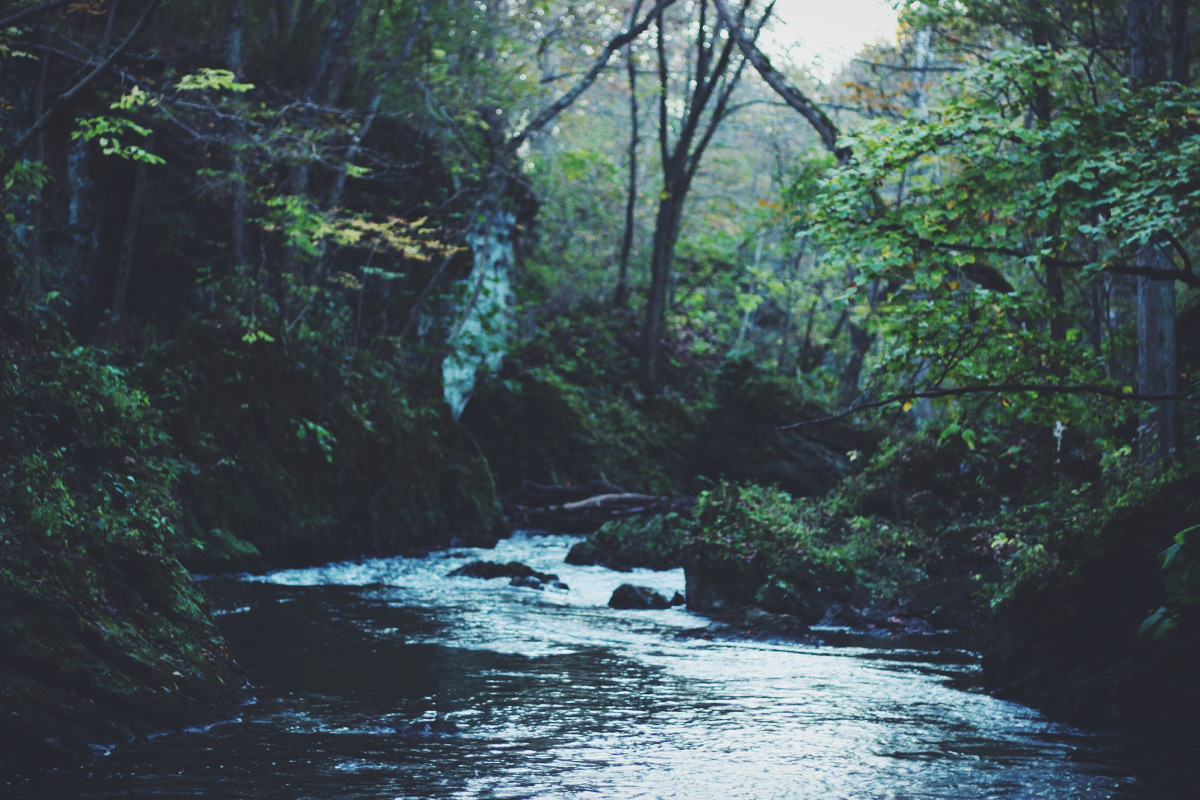
\includegraphics[width=\linewidth]{stream}
\caption{Legend (350 words max). Example legend text.}
\label{fig:stream}
\end{figure}

\begin{table}[ht]
\centering
\begin{tabular}{|l|l|l|}
\hline
Condition & n & p \\
\hline
A & 5 & 0.1 \\
\hline
B & 10 & 0.01 \\
\hline
\end{tabular}
\caption{\label{tab:example}Legend (350 words max). Example legend text.}
\end{table}

Figures and tables can be referenced in LaTeX using the ref command, e.g. Figure \ref{fig:stream} and Table \ref{tab:example}.

\end{document}